{\documentclass[authoryear]{elsarticle}

\setlength\arraycolsep{2pt}
\setlength{\parskip}{1ex plus 0.5ex minus 0.2ex}
\usepackage{graphicx}
\usepackage{amsfonts}
\usepackage{multirow}
\usepackage{comment}

%\usepackage{chicago}
\bibliographystyle{chicago}





\newcommand{\tr}{\mathrm{tr}}
\newcommand{\e}{\mathrm{e}}
\newcommand{\de}{\mathrm{d}}






%\renewcommand{\labelenumi}{(\roman{enumi})}

\newcommand{\cq}{,\quad }
\newcommand{\qq}{\quad \Rightarrow \quad}

%REFERENCES
\newcommand{\eref}[1]{(\ref{#1})}
\newcommand{\fref}[1]{Figure \ref{#1}}
\newcommand{\sref}[1]{\S\ref{#1}}
\newcommand{\tref}[1]{Table \ref{#1}}
\newcommand{\aref}[1]{\ref{#1}}


%notation for this paper

%EXPECTATIONS AND VARIANCES
\newcommand{\var}{{\rm var}}
\newcommand{\cov}{{\rm cov}}
\newcommand{\cor}{\mathrm{cor}}
\newcommand{\E}{{\mathrm E}}
\newcommand{\p}{{\mathrm P}}
\newcommand{\Ex}{{\mathcal E}}

%DENSITIES
\newcommand{\ft}{{\tilde{f}}}
\newcommand{\Ft}{{\tilde{F}}}




\newcommand{\bi}{\begin{itemize}}
\renewcommand{\i}{\item}
\newcommand{\ei}{\end{itemize}}



\begin{document}


\begin{frontmatter}

\title{Mean and risk decomposition with applications in capital and risk management}
\author[acst]{Weihao Choo\corref{cor1}}
\ead{weihao.choo@mq.edu.au}
\author[acst]{Piet de Jong}



\address[acst]{Department of Actuarial Studies Macquarie
University, NSW 2109, Australia.}
\cortext[cor1]{Corresponding author}




\begin{abstract}
This paper proposes a framework to analyze mean and risk across layers of loss. Loss layers characterise coverages in property and casualty insurance and reinsurance. The framework yields optimal pricing, risk and capital decisions.

Everything is a function of VaR spacings


\end{abstract}

\begin{keyword}
Layers, distortion, value-at-risk, spacing, excess-of-loss, mean density, risk density.
\end{keyword}



\end{frontmatter}



\section{Introduction and motivating example}\label{sintroduction}


Consider $100$ ordered observations of an insurance loss $x$: $\ell_1<\ell_2<\ldots<\ell_{100}$. The statistics $\ell_{i+1}-\ell_i$ and $(100-i)(\ell_{i+1}-\ell_i)$ are called the spacing and normalised spacing, respectively, in the order statistics \citep{shaked2007stochastic}. Spacings are of interest in engineering, for example corresponding to elapsed times between successive  failures of components forming a system.  

This paper uses spacings  to analyse mean and risk over layers of an insurance loss. The analysis yields solutions to common pricing, risk and capital decisions.  The framework  develops and exploits the following straightforward result for the sample mean of $x$:
\begin{equation}\label{mean}
\bar{x}=   \ell_1 + \frac{99}{100} (\ell_2-\ell_1) +\ldots + \frac{100-i}{100} (\ell_{i+1}-\ell_i)+\ldots +\frac{1}{100}(\ell_{100}-\ell_{99})  \;.
\end{equation}
 Define the mean of layer $[\ell_i,\ell_{i+1}]$ as 
$$
m_i \equiv \left(\frac{100-i}{100}\right) (\ell_{i+1}-\ell_i)\ ,
$$
then  $m_i$ is the spacing $\ell_{i+1}-\ell_i$ multiplied by the proportion or probability  $1-i/100$ of an observation exceeding $\ell_i$.  Adding up all $m_i$  yields the overall mean $\bar{x}$.  A layer is a portion of every loss outcome crossing an interval.

Loss layers are important quantities in insurance and reinsurance, particularly for property and casualty. Typical insurance and excess--of--loss reinsurance cover the loss layer between an excess and a limit. Capital shortfall is the loss layer starting from available capital. Layer means, and risks, are  critical inputs to pricing, capital and risk decisions. Further  loss layer discussion is in \cite{salzmann1963rating}, \cite{evans2001exposure} and \cite{wang1996pct} .

The following are important and exploitable points of the above setup:
\bi

\i Two  factors drive the magnitude  of $m_i$:   the exceedance  probability   $1-i/100$ and spacing $\ell_{i+1}-\ell_i$.  The exceedance probability decreases  with $i$.   The spacing may increase or decrease.   If the distribution is right skewed, as is typical for insurance losses, increasing $i$, leads to increased spacings.   Greater skewness implies larger spacings.    The overall behaviour of $m_i$ characterises the shape of the loss distribution.

\i Loss layers are expressed using sample values representing empirical percentiles or values-at-risk (VaRs) of $x$. For example the top 5 loss layer covers losses above the $95$th percentile. In contrast, current literature expresses loss layers in absolute amounts, for example between 1 and 2 million dollars. VaR layers are considered in this paper as they adjust to the shape and scale of the loss distribution, and can be interpreted probabilistically.

\i Individual layer means $m_i$ are building blocks for assessing expected coverage and related quantities. For example $m_1+m_2+\ldots+ m_{75}$ is the mean insured loss if coverage is limited to the 75th percentile. The sum $m_{95}+m_{96}+m_{97}+m_{98}+m_{99}$ is the mean of excess losses above the $95$th percentile, and represents the expected shortfall if capital is held at the $95$th percentile, or the expected excess-of-loss reinsurance coverage above the $95$th percentile.


\i The risk-adjusted layer mean replaces the exceedance probability $1-i/100$ in $m_i$ with a distorted probability $1-\Phi(i/100)$, yielding
$$
\tilde{m}_i = \left\{1-\Phi\left(\frac{i}{100}\right)\right\} (\ell_{i+1}-\ell_i)\ .
$$
Distorted probabilities shape layer means, yield distorted risk measures \citep{wang1996pct}  and are used in cumulative prospect theory \citep{tversky1992apt}.

\ei
Layer means and risks form a framework to optimise pricing, capital and risk decisions. Focus is usually placed on layers with large mean or risk. The framework provides  solutions and insights to insurance and also financial problems which may be difficult to express and solve using existing statistical methods.



Remaining sections of this paper are structured as follows. Sections \aref{smeansetup} to \aref{smeaneg} formalise and discuss layer means or ``mean densities." Risk densities are covered in sections \aref{srisksetup} to \aref{sriskeg}. Remaining sections apply mean and risk densities to optimise pricing, risk and capital decisions.



\section{VaR layers}\label{smeansetup}

This paper formalises and develops the example in \sref{sintroduction} for a continuous random loss $x\geq 0$ with distribution function $F$. Define the $\alpha$-Value-at-Risk (VaR) of $x$ as $V_\alpha\equiv F^-(\alpha)$ for $0\leq\alpha\leq 1$, where $F^-$ is the inverse distribution function of $x$.  Then  (should the inequality be strict or non strict?)
\begin{equation}\label{varlayer}
x=\int_0^1 (x>V_\alpha)\de V_\alpha =  \int_0^1 \ell_\alpha \de \alpha = \int_0^1\de L_\alpha  \cq \ell_\alpha\equiv (x>V_\alpha)V_\alpha'\;,
\end{equation}
where $(x>V_\alpha)$ is the indicator function: equal to one if $x>V_\alpha$ and zero otherwise, and $V_\alpha'$ is the derivative of $V_\alpha$ with respect to $\alpha$.   The proof of the first relation in \eref{varlayer} follows from
$
x=\int_0^x  1\de k = \int_0^\infty(k\le x)\de k 
$ and a change in the variable of integration.  Further  write
\begin{equation}\label{Xalpha}
L_\alpha \equiv \int_0^\alpha \ell_\beta\de \beta = \int_0^{\min\{\alpha,F(x)\}}\de V_\beta = \min(V_\alpha,x)\ .
\end{equation}

The VaR layer corresponding to percentile interval $[\alpha,\beta]$ is defined as 
$$
L_\beta-L_\alpha = \min(V_\beta,x)-\min(V_\alpha,x)\ .
$$ 
\fref{fix} plots a typical VaR layer as a function of $x$ on both the $x$ and percentile scale.   For small  intervals $[\alpha,\alpha+\de\alpha]$ the VaR layer is 
$$
\de L_\alpha \approx L_{\alpha+\de\alpha}-L_\alpha =\ell_\alpha \de\alpha = (x>V_\alpha)V_\alpha'\de\alpha\ ,
$$
called the $\mathrm{VaR}_\alpha$ layer and corresponds to the layer $[\ell_{i+1},\ell_i]$ in \sref{sintroduction}.  The $\mathrm{VaR}_\alpha$ layer has width $V_\alpha'\de\alpha\approx V_{\alpha+\de\alpha}-V_\alpha $ and  $V_\alpha'$ is called the VaR--spacing,  the continuous analogue to the discrete spacing $\ell_{i+1}-\ell_i$ in \sref{sintroduction}.

VaR layers are important for insurance calculations. For example the 
$
\de L_\alpha 
$ 
layer is the insured loss for a policy with deductible $V_\alpha$ and limit $V_{\alpha+\de\alpha}$, or the reinsured loss under an excess--of--loss reinsurance arrangement. When capital $V_\alpha$ is held against loss $x$, then $L_1-L_\alpha$ is the capital shortfall and the $L_\alpha$ layer is the capital used. VaR layers also characterise losses. For example the $L_1-L_\alpha$ layer represents additional losses contributed by the highest $1-\alpha$ portion of possible outcomes.


From \eref{varlayer}, any random variable $x\ge 0$ can be thought of as a sum of  $\mathrm{VaR}_\alpha$ layers over $0\le\alpha\le 1$. This paper uses \eref{varlayer} to decompose the mean and risk of $x$ across VaR layers. As noted in \sref{sintroduction}, layers are important as they represent insurance and reinsurance coverages, and their mean and risk values are critical inputs to pricing, capital and risk management decisions.

Endpoints of VaR layers are VaRs or percentiles. VaR endpoints adjust to the shape and scale of the loss distribution. The probability of the loss reaching the $\mathrm{VaR}_\alpha$ layer is fixed at $\alpha$, hence the mean and risk of a VaR layer are comparable across loss distributions. 

\cite{wang1996pct} consider layers indexed on the absolute scale using 
$$
x=\int_0^x 1\de k=\int_0^\infty (x>k) \de k \;,
$$
hence the $k$-layer of $x$ is $(x>k)\de k$. The probability of reaching the $k$-layer is $1-F(k)$ and depends on $F$. As a result the means and risks of the $k$-layers are not comparable across loss distributions.

\section{The mean density}


The mean density  is defined analogous to \eref{mean}:
\begin{equation}\label{meancont}
m_\alpha \equiv \E(\ell_\alpha)=\E\left\{(x>V_\alpha)V_\alpha' \right\}
=(1-\alpha)V_\alpha'\cq 0\le\alpha\le 1\ ,
\end{equation}
where $\E$ is the expectation given $\alpha$ is uniform. The mean density $m_\alpha$ is the product of $1-\alpha$, the probability of $x$ reaching the $\mathrm{VaR}_\alpha$ layer, and the VaR-spacing $V_\alpha'$ measuring layer width. 

As $\alpha$ increases, $1-\alpha$ decreases reflecting reduced likelihood of reaching higher layers. On the other hand for a right skewed loss distribution,  $V_\alpha'$ increases  where the probability density is decreasing. The behaviour of the mean density depends on the relative movements in $1-\alpha$ and $V_\alpha'$. For example, the exponential distribution has a constant mean density whereas the Pareto distribution has an increasing mean density due to more rapidly increasing VaR spacings. Example mean densities are shown in \sref{smeaneg}.

Using \eref{varlayer},
$$
\int_0^1 m_\alpha \de \alpha = \E\left( \int_0^1 \ell_\alpha \de \alpha \right) = \E(x) \;.
$$
Integrating $m_\alpha$, and $\ell_\alpha$, over subsets of the unit interval yields mean values and values of layers representing for example insurance coverage with a deductible and limit. This result is discussed in the next section.


As mentioned above  \cite{wang1996pct} considers loss layers on the absolute scale and the $k$-layer is $(x>k)\de k$. The corresponding mean density is $\E\{(x>k)\}=1-F$ is the survival function. \cite{wang1996pct} calls $1-F$ the premium layer density.


Integrating the mean density over subintervals of $[0,1]$ yields the mean of the VaR layer over the interval:
\begin{equation}
\E(L_\beta-L_\alpha)= \E\left( \int_\alpha^\beta \ell_\pi \de\pi \right)=\int_\alpha^\beta m_\pi\de \pi \;,
\end{equation}
 representing, for example, the mean covered loss or pure premium under an insurance or reinsurance arrangement with deductible $V_\alpha$ and limit $V_\beta$, and the expected capital shortfall $(\alpha=\gamma,\beta=1)$ or capital usage $(\alpha=0,\beta=\gamma)$ when capital $V_\gamma$ is held against $x$.  The expectation is an important input to insurance and reinsurance pricing, and decisions on policy conditions, capital amounts to hold, and other risk and capital management strategies. Section \aref{srisksetup} discusses risk values of VaR layers, also a critical input to these decisions when volatility is of concern. Applications of mean and risk densities are discussed in sections \aref{sapplication} and beyond.

Example mean densities for common probability distributions are (In all cases $b>0$ is a scale parameter)
\bi
\i The  uniform distribution over $[0,b]$ yields
$$
V_\alpha=b\alpha \cq V_\alpha'=b \cq m_\alpha=(1-\alpha)b \;,
$$
and the mean density is linearly decreasing. Spacings are equal over all VaR layers, and losses are less likely to reach higher layers, hence the mean density is decreasing. The mean density is also proportional to scale, and this is case in general.  (Not sure I understand the last sentence).
\i The  exponential  with mean $b$ is
$$
F(x)=1-\e^{-x/b} \cq V_\alpha=-b \ln(1-\alpha) \cq V_\alpha'=\frac{b}{1-\alpha} \cq m_\alpha=b\;,
$$
and the mean density is constant since increasing VaR spacings exactly offset decreasing probabilities of reaching higher layers.

\i The  Pareto  with shape parameter $c>1$ is
$$
F(x)=1- \left(\frac{b}{b+x}\right)^c \cq V_\alpha= b\left\{(1-\alpha)^{-1/c}-1\right\} \;,
$$
$$
 V_\alpha'=\frac{b}{c (1-\alpha)^{1/(c+1)}} \cq m_\alpha = \frac{b}{c(1-\alpha)^{1/c}} \;.
$$
The mean density increases to infinity as $\alpha\rightarrow 1$:  increasing VaR spacing more than offsets decreasing probabilities.

\i The Weibull distribution with shape parameter $k>0$,
$$
F(x)=1-\e^{-(x/b)^k} \cq V_\alpha = b\left\{- \ln(1-\alpha)\right\}^{1/k} \;,
$$
$$
V_\alpha'=\frac{b\left\{-\ln(1-\alpha)\right\}^{1/(k-1)}}{k(1-\alpha)}  \cq
m_\alpha=\frac{b\left\{-\ln(1-\alpha)\right\}^{1/(k-1)}}{k} \;.
$$
Setting $k=1$ yields the exponential distribution and $m_\alpha=b$. Reducing $k$ increases skewness and yields increasing $m_\alpha$. Vice versa if $k>1$.


\ei
\fref{fmeancont} plots mean densities for the above distributions with parameters satisfying $\E(x)=1$. Hence mean densities in \fref{fmeancont} all integrate to one. For the exponential distribution, the overall mean value is spread uniformly across VaR layers. For the Pareto distribution, the bulk of the overall mean value is captured by higher VaR layers due to an increasing mean density. The opposite applies to the uniform distribution.
\begin{figure}
  \begin{center}
    \begin{tabular}{cc}
      \resizebox{120mm}{!}{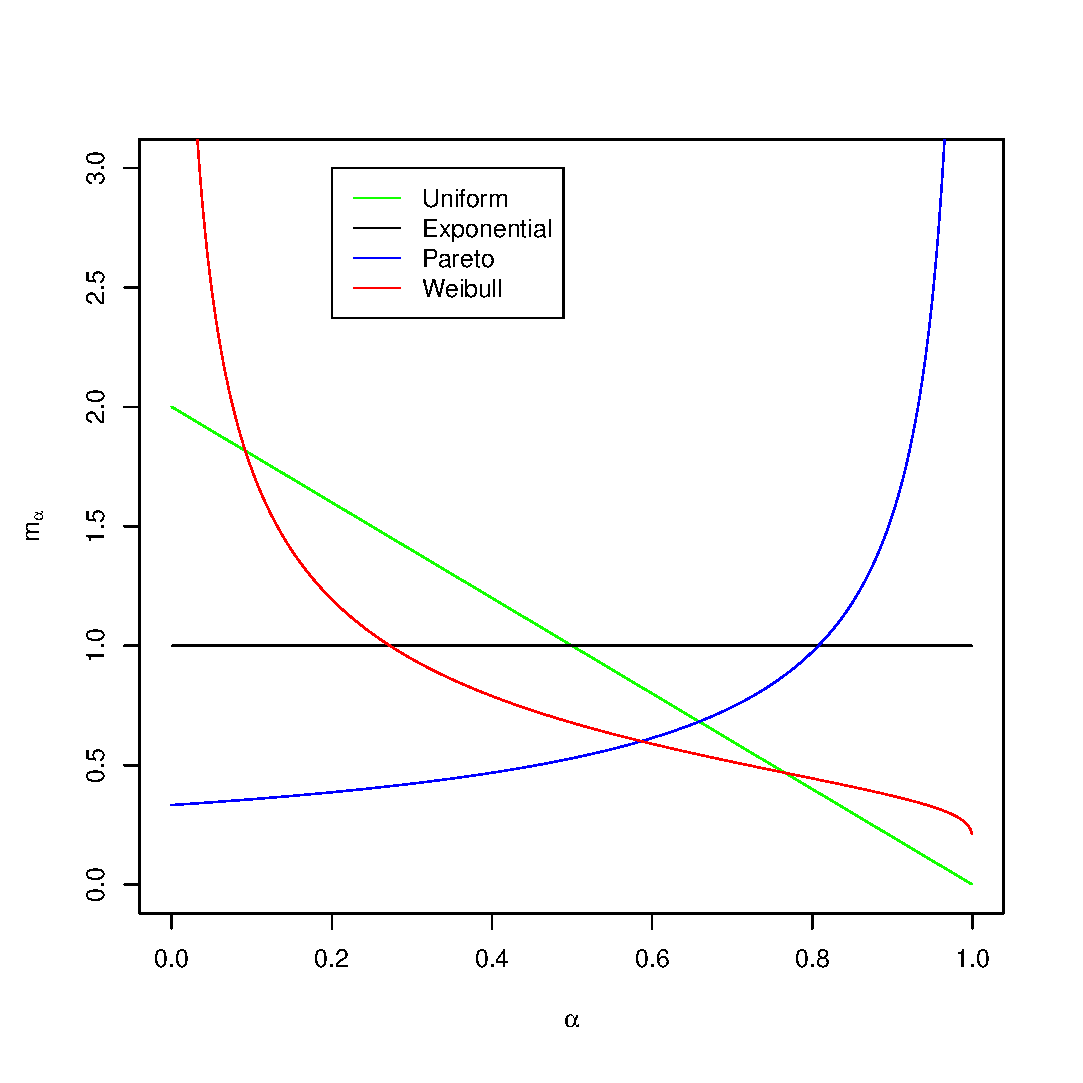
\includegraphics{meancont.eps}}
    \end{tabular}
    \caption{Mean densities for uniform ($b=2$), exponential ($b=1$), Pareto ($b=0.5$, $c=1.5$) and Weibull ($b=1.13$, $k=2$) distributions. The area underneath each curve is 1.}
    \label{fmeancont}
  \end{center}
\end{figure}

The constant mean density for the exponential distribution is a benchmark for assessing skewness of the loss distribution. A decreasing mean density (for example uniform distribution and Weibull distribution for $k>1$) implies VaR spacings increase at a lower rate compared to the exponential, and hence lower skewness. Vice versa for an increasing mean density (for example Pareto distribution and Weibull distribution for $k<1$). The mean density has derivative
$$
m'_\alpha=(1-\alpha)V_\alpha''-V_\alpha' \;,
$$
hence mean density is increasing if and only if $(1-\alpha)V_\alpha''/V_\alpha'>1$.


\section{Properties of mean densities}

The mean density $m_\alpha$ defined in \eref{meancont} is non-negative for any loss $x\geq 0$. Further  if $y=f(x)$ where $f>0$ is  increasing  then   
$$
V_\alpha(y)=f(V_\alpha)\cq m_\alpha(y) = (1-\alpha)f'(V_\alpha)V_\alpha'=m_\alpha f'(V_\alpha)\ .
$$
In particular if $y=f(x)=cx$ then $\mathrm{VaR}_\alpha(y)=cm_\alpha$.


The mean density uniquely characterises the loss distribution. Given $m_\alpha$ for all $0\leq \alpha \leq 1$, VaR spacings are $m_\alpha/(1-\alpha)$ which are then integrated to yield:
$$
V_\alpha = \int_0^\alpha \frac{m_t}{1-t} \de t  \;.
$$
Taking the inverse of the result yields the loss distribution $F$. Hence $\mathrm{VaR}_\alpha$ is the integral of scaled mean density $m_t$ up to $t=\alpha$ with scaling factor $1/(1-t)$. Higher values of $m_t$, especially over $t$ closer to $\alpha$, implies higher $\mathrm{VaR}_\alpha$.



The mean density at $\mathrm{VaR}_\alpha$ layer of $x$ is the reciprocal of the hazard rate at $\mathrm{VaR}_\alpha$:
$$
m_\alpha = \left(\lambda_{V_\alpha}\right)^{-1}  \cq \lambda_x\equiv \frac{f(x)}{1-F(x)} \;,
$$
where $f\equiv F'$ is the loss density. The result follows by noting $F(V_\alpha)=\alpha$ and $V_\alpha'=1/f(V_\alpha)$. The hazard rate at say $\ell_0$ indicates the probability of $x=\ell_0$ given $x>\ell_0$. \cite{hogg2009loss} further discusses hazard rates.





\section{Distortion risk and risk density}\label{srisksetup}

Previous sections discuss mean values of loss layers, where loss layers represent for example insurance or reinsurance coverage with limits and deductibles, and capital usage or shortfall. This section discusses risk values of loss layers, where risk is measured using distortion. Mean and risk values together form critical inputs to decision making around pricing, capital and risk management.

\cite{wang1996pct} replaces the distribution function $F$ with distorted $\Phi\circ F$ where $\Phi$ is an increasing, convex distortion operator satisfying $\Phi(0)=0$ and $\Phi(1)=1$. Distortion risk is the difference between mean values computed under distorted and original distributions. Hence the distortion risk of $x$ is
$$
\Ex(x)-\E(x)=\int_0^\infty \left[ 1-\Phi\{F(x)\} \right] \de x - \int_0^\infty \{ 1-F(x)\} \de x
$$
$$
=\int_0^\infty \left[ F(x)-\Phi\{F(x)\} \right] \de x  \;.
$$
where $\Ex$ calculates expectations using the distorted $\Phi\circ F$. Distortion risks are positive since $\Phi$ is convex thus $\Phi\{F(x)\}<F(x)$ for all $x$. Applying integration by parts to the first integral above yields the alternative expression
$$
\Ex(x)-\E(x)= \E\left\{ x\Phi'(u) \right\} - \E(x) =\cov\left\{x,\Phi'(u) \right\}
$$
$$
= \sigma_x \sigma_{\Phi'} \cor\left\{x,\Phi'(u) \right\} \cq u\equiv F(x) \;,
$$
which is the loss aversion premium \citep{choo2009loss}, where $\cov$ and $\cor$ compute covariance and correlation under $F$, and $\sigma_x$ and $\sigma_\phi$ are standard deviations. Therefore distortion risk and loss aversion premium are equal and both driven by the volatility of $x$ and other factors depending on $\Phi$.

Distortion risks are important inputs to decisions where volatility is of concern. For example distortion risks form premium loadings and capital buffers on insurance losses, and risk premiums on investment returns. Mean values are insufficient as they do not capture the spread and skewness of the distribution of outcomes. Applying various distortion operators generates different distortion risk measures. Examples are discussed in \cite{wang1995insurance}, \cite{wang2000cdo} and \cite{choo2009loss}, and include the proportional hazards risk, conditional-tail-expectation and expected-maximal-loss.

The risk density yields the distortion risk of various VaR layers and is again the difference between distorted and original mean values:
\begin{equation}\label{riskcont}
r_\alpha \equiv \Ex(\ell_\alpha)-\E(\ell_\alpha) = \{1-\Phi(a)\}V_\alpha'-(1-\alpha)V_\alpha'=\{\alpha-\Phi(\alpha)\}V_\alpha'
\end{equation}
noting the distorted probability of $x>V_\alpha$ is $1-\Phi\{F(V_\alpha)\}=1-\Phi(\alpha)$. This distorted probability exceeds the original probability $1-\alpha$ since $\Phi$ is convex. Therefore distortion increases the probability of $x$ reaching any VaR layer, and the risk density is proportional to the amount of increase. The increase $\alpha-\Phi(\alpha)$ represents the extent of distortion at $\alpha$.

Also note end points of VaR layers are unchanged at $V_\alpha=F^-(\alpha)$, even though the $\mathrm{VaR}_\alpha$ of the distorted distribution is $F^-\{\Phi^-(\alpha)\}$. Therefore end points of VaR layers are fixed and specified using the original distribution, and distortion only affects the probability of the loss reaching various layers.

Similar to $m_\alpha$, integrating $r_\alpha$ over all $\alpha$ yields the distortion risk of $x$:
$$
\int_0^1 r_\alpha \de \alpha = \int_0^1 \{\Ex(\ell_\alpha)-\E(\ell_\alpha)\} \de \alpha = \Ex(x)-\E(x) \;.
$$
Alternatively, $\mathrm{VaR}_\alpha$ layers for all $\alpha$ are comonotonic, and distortion risks of comonotonic random variables are additive \citep{wang1997aci}. In addition integrating the risk density over $[a,b]$ yields the risk of the $[a,b]$-VaR layer:
$$
R_{[a,b]} \equiv \int_a^b r_\alpha \de \alpha = \Ex\left(L_{[a,b]}\right)-\E\left(L_{[a,b]}\right)  \;.
$$
For example $R_{[a,b]}$ is the risk of an insured loss $x$ with deductible $V_a$ and limit $V_b$. The premium for this insured loss is then $L_{[a,b]}+\theta R_{[a,b]}$ where $\theta>0$ is a profit margin.  $R_{[0,b]}$ is the risk of losses capped at $V_b$, and $R_{[a,1]}$ is the risk of losses in excess of $V_a$. These two risks are important inputs when setting capital for example. The risk density spreads the overall risk of $x$ across VaR layers and focus is generally placed on higher risk layers to form optimal decisions. Applications of mean and risk densities are further discussed in \sref{sapplication}.

Similar results as \eref{differentiate} apply to $M_{[a,b]}$:
$$
\frac{\partial}{\partial b} R_{[a,b]} = r_b \cq \frac{\partial}{\partial a} R_{[a,b]} = -r_a \;.
$$










\section{Risk ratios}


The risk ratio is the ratio between risk and mean densities:
\begin{equation}\label{riskratio}
r_\alpha^* \equiv \frac{r_\alpha}{m_\alpha} = \frac{\{\alpha-\Phi(\alpha)\}V_\alpha'}{(1-\alpha)V_\alpha'} = \frac{\alpha-\Phi(\alpha)}{1-\alpha} \;.
\end{equation}
Risk ratios indicate the level of risk relative to mean for every VaR layer. Risk ratios depend entirely on the distortion operator $\Phi$. Risk ratios are independent of the loss distribution since VaR spacing $V_\alpha'$ is a multiplicative factor in both $r_\alpha$ and $m_\alpha$, and cancels after division. 

Risk ratios are larger at higher layers, since the derivative of $r_\alpha^*$ with respect to $\alpha$ is given by
$$
\frac{\de}{\de \alpha}r_\alpha^* = \frac{1-\Phi(\alpha)-(1-\alpha)\Phi'(\alpha)}{(1-\alpha)^2} \geq 0 \;.
$$
The inequality holds since $1-\Phi(\alpha)=\int_\alpha^1 \Phi'(u) \de u\geq \int_\alpha^1 \Phi'(\alpha)\de u=(1-\alpha)\Phi'(\alpha)$ noting $\Phi$ is convex implying $\Phi'$ is increasing. Thus higher VaR layers are riskier than lower VaR layers as a proportion of mean values. End points of risk ratios are $r_0^* = 0$ and $r_1^*=\Phi'(1)-1$. Relative risk is zero at the bottom VaR layer, and increases to $\Phi'(1)-1$ at the top VaR layer.



Given individual risk ratios, the overall risk and risk ratio of any VaR layer $L_{[a,b]}$ is computed as
$$
R_{[a,b]} = \int_a^b r_\alpha^* m_\alpha \de \alpha
\cq \frac{R_{[a,b]}}{M_{[a,b]}} = \frac{\int_a^b r_\alpha^* m_\alpha \de \alpha }{\int_a^b   m_\alpha \de \alpha}\;.
$$
Hence the overall risk ratio is a weighted average of individual risk ratios, with weights given by mean density values. Given the overall mean $M_{[a,b]}$, the overall risk ratio and hence risk are high if the mean density is larger at higher layers since larger risk ratios are then weighted more heavily. For example the Pareto has a higher risk and risk ratio than the uniform, exponential and Weibull due to an increasing mean density. Examples are further discussed in the next section.


The set of risk ratios $r_\alpha^*$ over $0\le\alpha\le 1$ uniquely characterises the distortion operator $\Phi$. Therefore an alternative formulation of $\Phi$ is to specify risk ratios across all VaR layers and then set
$$
\Phi(\alpha)=\alpha-(1-\alpha)r_\alpha^* \;.
$$
The condition $\Phi(0)=0$ requires $r_0^*=0$. Increasing and convex $\Phi$ respectively require $1+r_\alpha^*-(1-\alpha)(r_\alpha^*)'>0$ and $2(r_\alpha^*)'-(1-\alpha)(r_\alpha^*)''>0$.


\section{Example risk ratios and risk densities}\label{sriskeg}

The following are risk ratios based on distortion operators discussed in \cite{wang1995insurance} and \cite{choo2009loss}. As highlighted in the previous section, risk ratios only depend on the distortion operator. Multiplying risk ratios with the mean density yields the risk density.

\bi

\i Assume the distortion operator $\Phi(v)=(v>c)(v-c)/(1-c)$ where $0\leq c\leq 1$. The overall distortion risk of $x$ is the conditional-tail-expectation $\E(x|x>V_c)-\E(x)$, the expected value of losses above $c$-VaR in excess of the mean loss. The risk ratio is
$$
r_\alpha^*= (\alpha\leq c) \frac{\alpha}{1-\alpha}+(\alpha>c) \frac{c}{1-c} \;.
$$
Risk ratio in this case increases from zero until the $c$-VaR layer, and remains constant at $c/(1-c)$ for all higher layers. Larger $c$ yields higher risk ratios across all VaR layers, hence  $c$ indicates risk aversion.



\i Assume the power distortion operator $\Phi(v)=v^n$ where $n\geq 1$. If $n$ is an integer, the distortion risk is $\E\{\max(\ell_1,\ldots,\ell_n)\}-\E(x)$ or the expected-maximal-loss in excess of the mean loss, where $\ell_1,\ldots \ell_n$ are independent copies of $x$. The risk ratio in this case is
$$
r^*_\alpha =  \frac{\alpha -\alpha^n}{1-\alpha} =  \sum_{i=1}^{n-1} \alpha^i \;,
$$
where the final expression assumes integer $n$, and is a polynomial of degree $n-1$ with unit coefficients. Larger $n$ yields higher risk ratios for all $\alpha$, hence $n$ indicates risk aversion.


\i Assume the proportional hazards transform, $\Phi(v)=1-(1-v)^{1/\gamma}$ where $\gamma\geq 1$. The distortion risk is $\int_0^\infty \{S(x)\}^{1/\gamma} \de x-\int_0^\infty S(x) \de x$ where $S$ is the survival function. The risk ratio is
$$
r_\alpha^*=\frac{\alpha-\{1-(1-v)^{1/\gamma}\}}{1-\alpha} = (1-\alpha)^{1/\gamma-1}-1 \;.
$$
Higher $\gamma$ increases risk ratios.

\ei
The four panels in \fref{frisk} graph mean and risk densities using a power distortion operator $\Phi(v)=v^3$ and loss distributions in \fref{fmeancont}. The risk ratio is $r_\alpha^*=\alpha(1+\alpha)$. For the uniform loss distribution, risk is highest around median VaR layers since increasing risk ratios are applied to a decreasing mean density. Risk is generally higher at higher VaR layers for the exponential, Pareto and Weibull loss distributions. Pareto has the highest overall risk, since higher risk ratios are applied to higher mean densities at higher VaR layers. Pareto has an increasing mean density due to its skewness.

\begin{figure}
  \begin{center}
    \begin{tabular}{cc}
      \resizebox{60mm}{!}{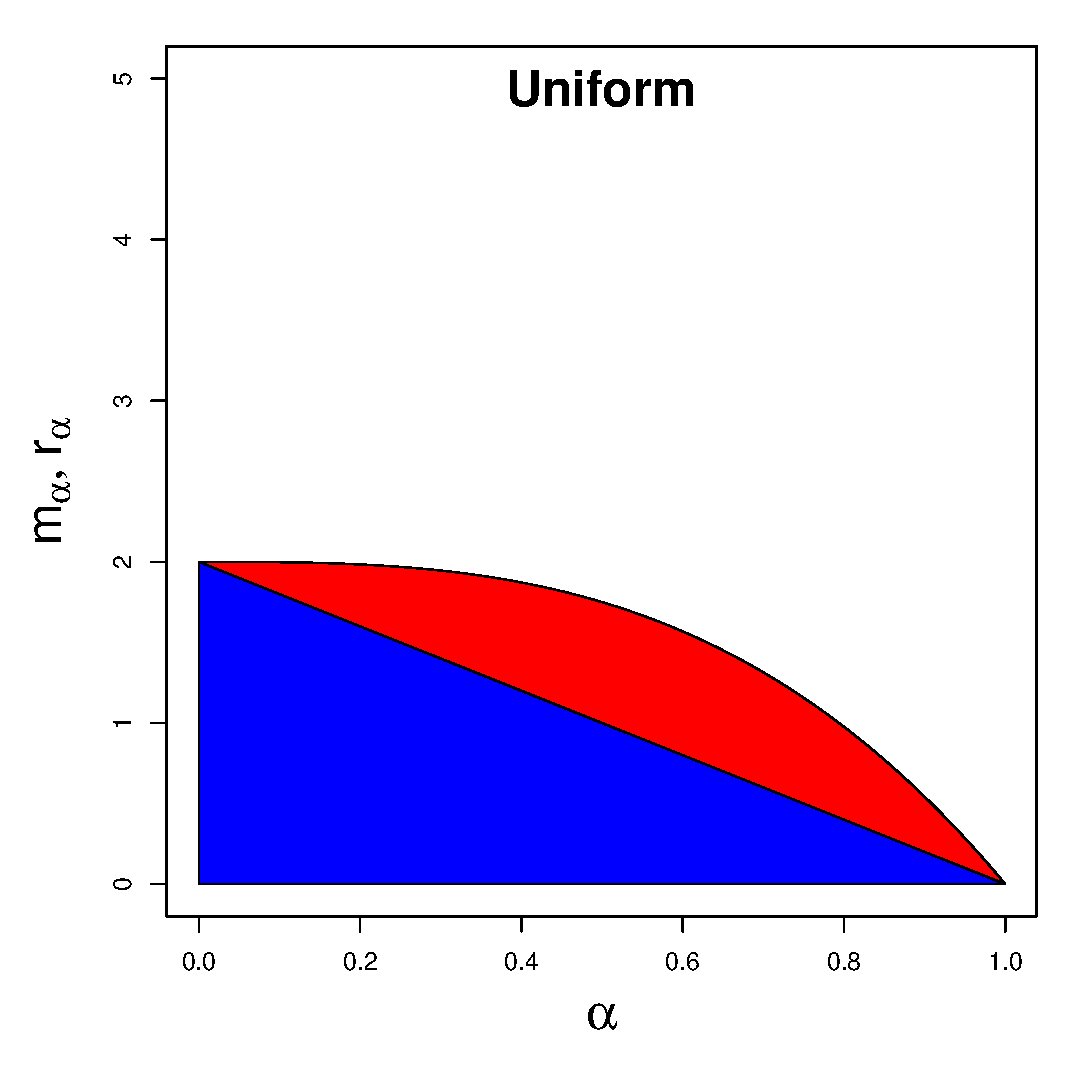
\includegraphics{unirisk.eps}}
      \resizebox{60mm}{!}{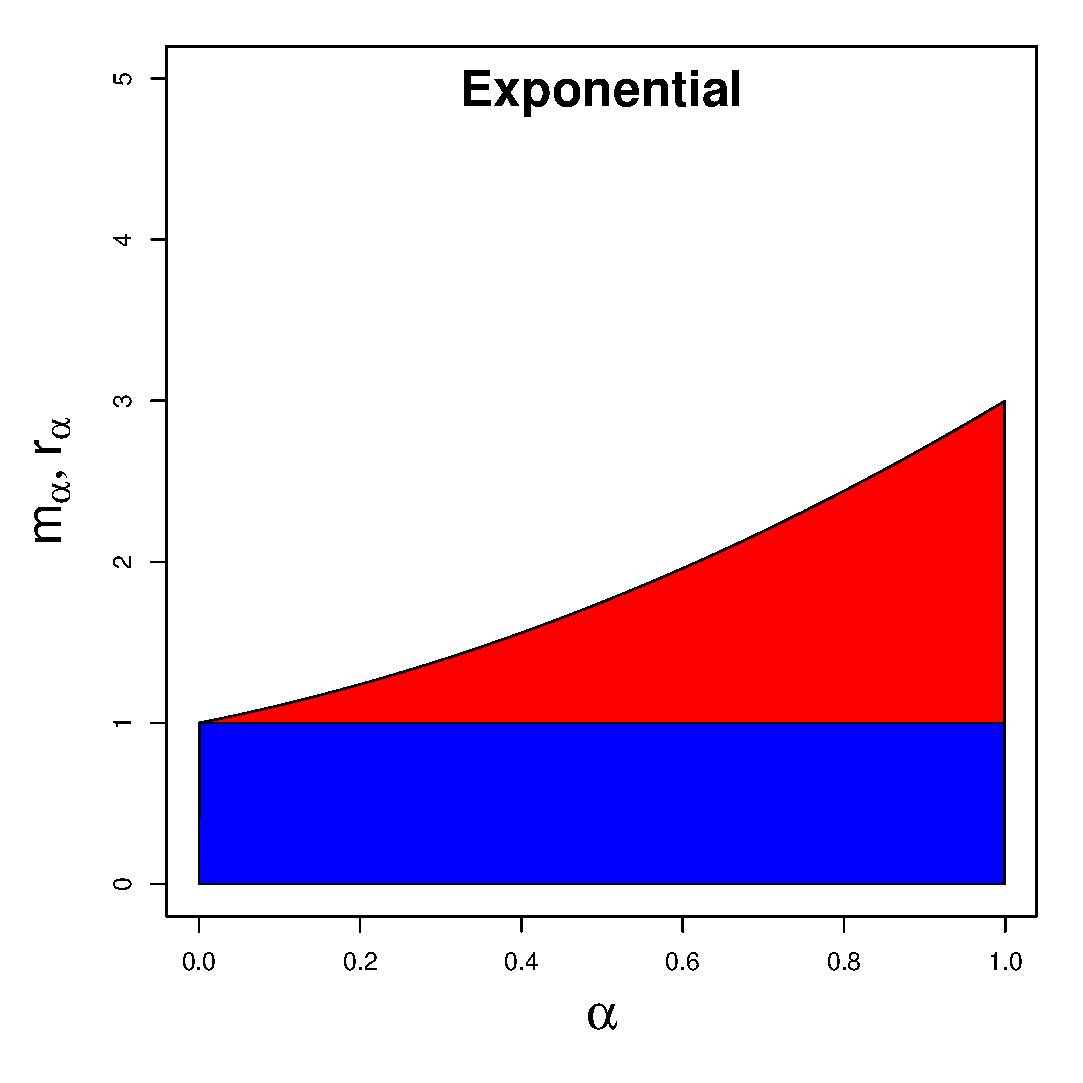
\includegraphics{exprisk.eps}} \\
      \resizebox{60mm}{!}{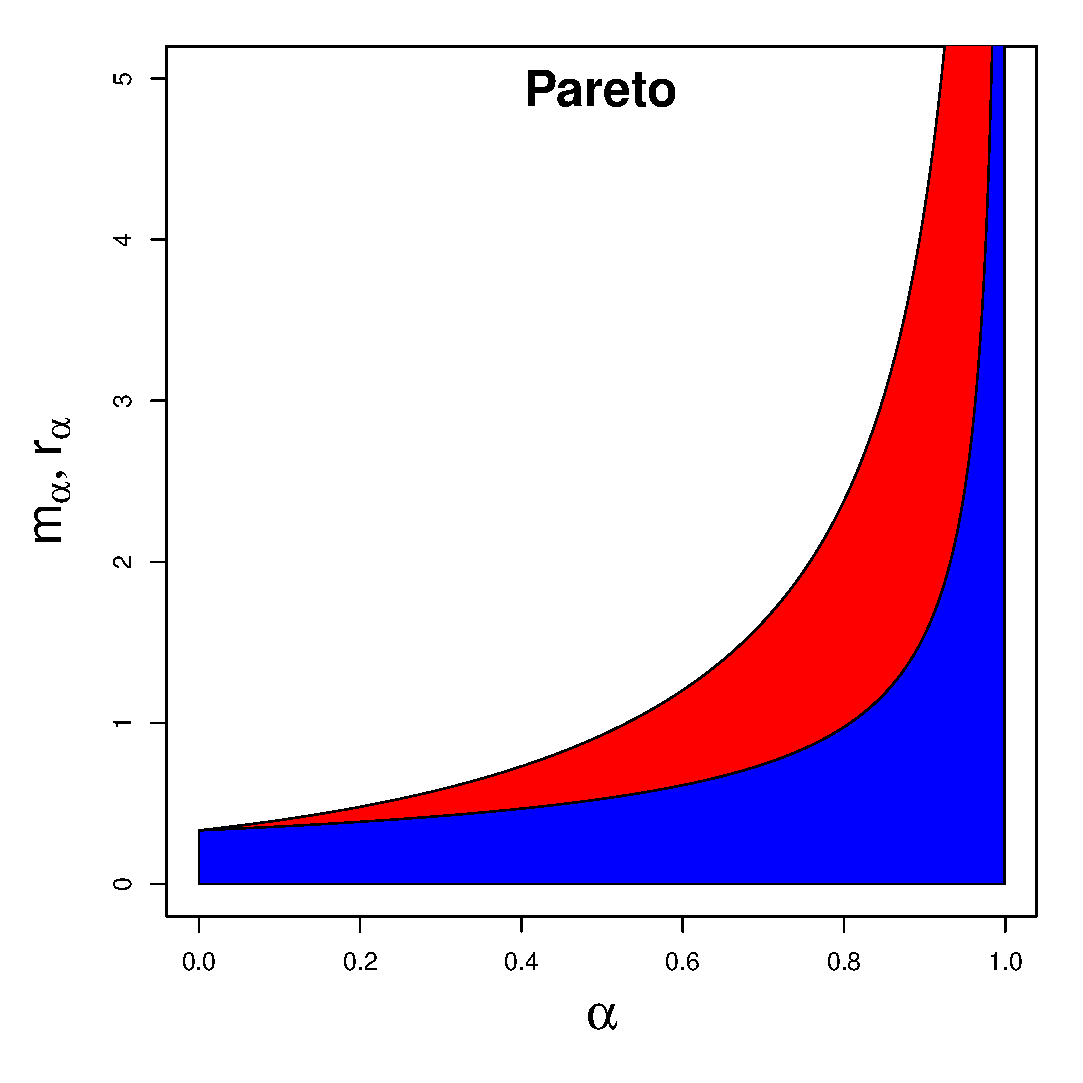
\includegraphics{parrisk.eps}}
      \resizebox{60mm}{!}{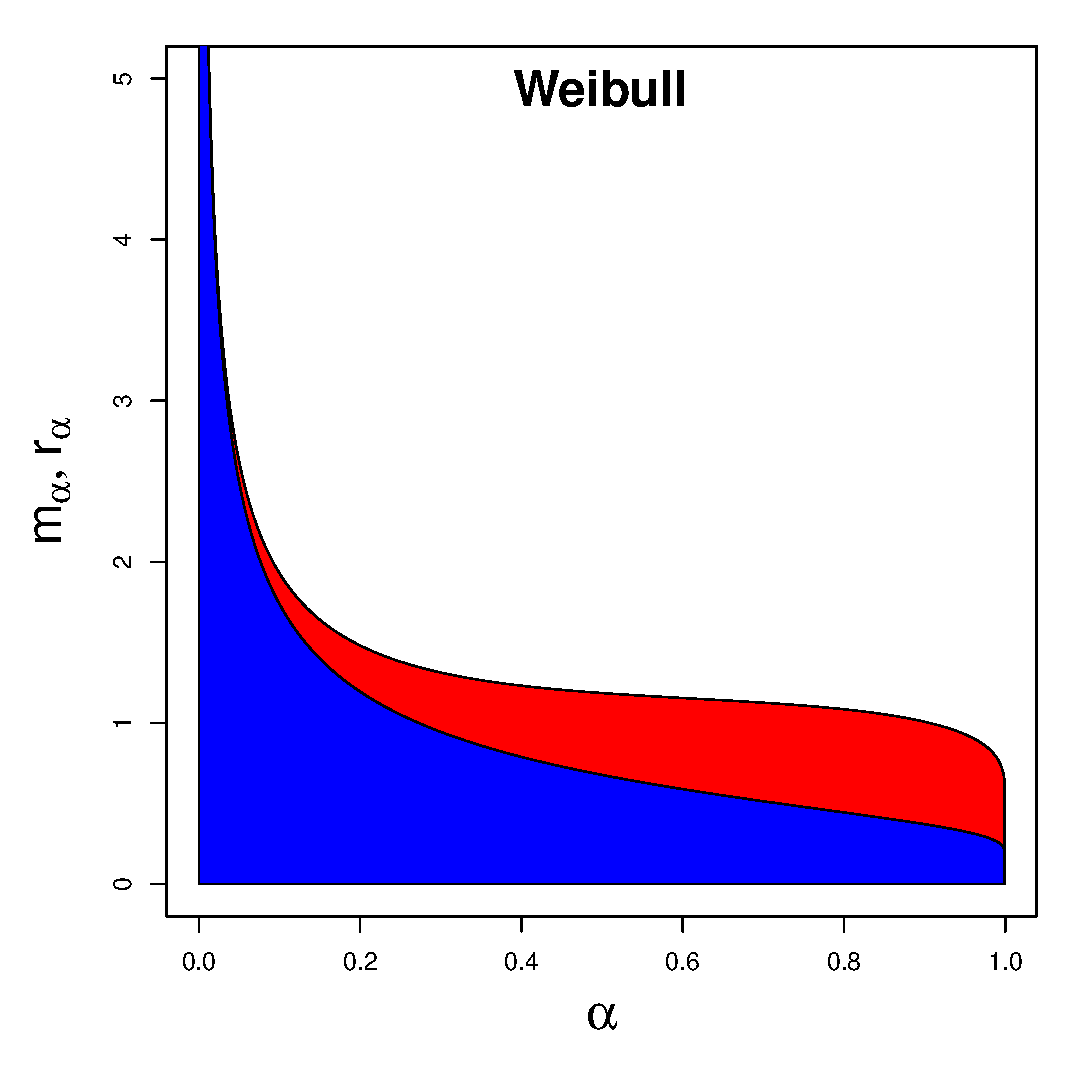
\includegraphics{weirisk.eps}} \\
    \end{tabular}
    \caption{Mean densities (blue area) and risk densities (red area) for the $4$ loss distributions in \fref{fmeancont}. The distortion operator is $\Phi(v)=v^3$ and the risk ratio is $r_\alpha^*=\alpha(1+\alpha)$. }
    \label{frisk}
  \end{center}
\end{figure}




\section{Volatility density and volatility ratio}\label{svolatility}


Volatility densities are similar to risk densities and indicate the volatility of each VaR layer. Volatility is measured by standard deviation. Unlike risk densities, volatility densities do not integrate to the overall loss standard deviation. This paper focuses on risk densities due to their additivity. In addition distortion risk captures the skewness of loss distributions, and standard deviation is a more appropriate risk measure for symmetric distributions.

The volatility density is the standard deviation of $\ell_\alpha$:
\begin{equation}\label{volatility}
s_\alpha \equiv \sqrt{\var(\ell_\alpha)} = \sqrt{\alpha(1-\alpha)}V_\alpha' \;,
\end{equation}
since the $\mathrm{VaR}_\alpha$ layer is Bernoulli distributed with probability $1-\alpha$ and scale $V_\alpha'$. The volatility ratio is the ratio between volatility and mean densities:
$$
s_\alpha^* \equiv \frac{s_\alpha}{m_\alpha} = \frac{\sqrt{\alpha(1-\alpha)}V_\alpha'}{(1-\alpha)V_\alpha'} = \sqrt{\frac{\alpha}{1-\alpha}} \;,
$$
and is the coefficient of variation of $\ell_\alpha$. Similar to risk ratios, volatility ratios are increasing and are independent of the loss distribution. Volatility ratio starts at zero at the bottom VaR layer, and increases to infinity at the top VaR layer.

Integrating $s_\alpha$ over $[a,b]$ yields the volatility of the $[a,b]$-VaR layer:
$$
S_{[a,b]} \equiv \int_a^b \sqrt{\alpha(1-\alpha)}V_\alpha' \de \alpha
= \sqrt{b(1-b)}V_b-\sqrt{a(1-a)}V_a
$$
$$
- \int_a^b \frac{0.5-\alpha}{\sqrt{\alpha(1-\alpha)}} V_\alpha \de\alpha \;.
$$
The first integral above is a weighted sum of VaR spacings between $a$-VaR and $b$-VaR, where weights are symmetric about, and highest at, the median. Larger $S_{[a,b]}$ implies greater volatility over the $[a,b]$-VaR layer. In addition $S_{[a,b]}$ is an upper bound on the standard deviation of the $[a,b]$-VaR layer:
\begin{equation}\label{bound}
\sqrt{\var\left( L_{[a,b]}\right)} \le S_{[a,b]}  \;,
\end{equation}
since the standard deviation of a sum ($L_{[a,b]}$) is less than the sum of standard deviations ($S_\alpha$). VaR layers are comonotonic but not linearly dependent, hence equality in \eref{bound} does not hold in general.

When $a=0$ and $b=1$ the integral of the volatility density is
$$
S_{[0,1]} = \int_0^1 \frac{\alpha-0.5}{\sqrt{\alpha(1-\alpha)}} V_\alpha \de\alpha  = \int_{0.5}^1 \frac{\alpha-0.5}{\sqrt{\alpha(1-\alpha)}} \left(V_\alpha-V_{1-\alpha} \right) \de \alpha \ge \sqrt{\var(x)} \;.
$$
Hence overall loss volatility as measured by the volatility density is the weighted difference between VaRs above and below the median, and in general exceeds the loss standard deviation.








\section{Calculation using simulation losses}

Previous sections define mean, risk and volatility densities for a continuous loss random variable. It is common for insurance and financial companies to simulate future outcomes to make decisions. Given an ordered sample of simulated losses $\ell_1,\ldots,\ell_n$, calculate mean, risk and volatility densities as follows:
\bi
\i Set VaRs equal to ordered observations: $V_{i/n}=\ell_i$. The $i/n$-VaR layer is $(x>\ell_i)(\ell_{i+1}-\ell_i)$ where $x$ is random.

\i The mean density is $m_{i/n}=(1-i/n)V_{i/n}'$, for $i=0,\ldots,n-1$ where the derivative $V_{i/n}'=n(V_{(i+1)/n}-V_{i/n})$ and $V_0=0$.

\i Risk ratios are computed using the specified distortion operator: $r_{i/n}^*=\{i/n-\Phi(i/n)\}/(1-i/n)$. The risk density is $r_{i/n}=m_{i/n}*r_{i/n}^*$.

\i Volatility ratios are $s_{i/n}^*=\sqrt{(i/n)/(1-i/n)}$. The volatility density is the product $s_{i/n}=m_{i/n}*s_{i/n}^*$.
\ei
Overall mean, risk and volatility are the respective sums (rather than integrals)
$$
\sum_{i=0}^{n-1} \frac{m_{i/n}}{n} \cq \sum_{i=0}^{n-1} \frac{r_{i/n}}{n} \cq
\sum_{i=0}^{n-1} \frac{s_{i/n}}{n}\;.
$$
Taking sums over other subsets yield mean, risk and volatility over corresponding VaR layers. Manipulating the first summation above yields the arithmetic mean $\sum_{i=1}^n \ell_i /n$.



\section{Applications}\label{sapplication}

Remaining sections of this paper apply mean and risk densities to common problems in risk and capital management. Existing statistical tools provide identical solutions to some of the problems. However mean and risk densities offer a more elegant solution, and yield additional insights.

Capital covers adverse loss outcomes. Capital is usually set equal to VaR with a fixed threshold. For example Solvency II insurance regulation references $90\%$ and $99.5\%$ VaRs \citep{eling2007solvency}. VaR based capital limits the probability of shortfall -- $10\%$ and $0.5\%$ respectively in Solvency II. VaR based capital adjusts to the shape and scale of the loss distribution. Given a fixed threshold, VaR increases with scale and skewness of the loss distribution.

Conflicting considerations are involved when deciding how much capital to hold. Higher capital reduces the probability and extent of a shortfall. However holding capital involves an opportunity cost. An optimal capital amount balances shortfall and opportunity cost.

Higher risk requires more capital. Understanding key sources of risk yields optimal risk management decisions to reduce required capital, such as reinsurance purchase and limiting loss coverage.



\section{Pricing loss layers}

The following applies mean and risk densities to pricing loss layers. Given loss $x$, suppose the layer $L_{[a,b]}$ is insured (or reinsured). Hence $V_a$ is the deductible or excess and $V_b$ is the limit. The payout is $x-V_a$ if $x>V_a$, and is capped at $V_b-V_a$. The premium is
$$
M_{[a,b]}+ R_{[a,b]} = \int_a^b (m_\alpha+r_\alpha) \de \alpha = \int_a^b \{1-\Phi(\alpha) \} V_\alpha' \de \alpha
$$
$$
= \{1-\Phi(b)\}V_b-\{1-\Phi(a)\}V_a + \int_a^b V_\alpha \phi(\alpha) \de \alpha  \;,
$$
where $M_{[a,b]}$ is the pure premium and $R_{[a,b]}$ is the risk loading. Incremental premium changes from changing the deductible and the limit are respectively given by derivatives
$$
\frac{\partial}{\partial a} \left\{  M_{[a,b]}+ R_{[a,b]}  \right\} = -(m_a+ r_a)
\cq \frac{\partial}{\partial b} \left\{  M_{[a,b]}+  R_{[a,b]}  \right\} = m_b+ r_b
\;.
$$
Refer to mean and risk densities in \fref{frisk}. The premium $M_{[a,b]}+ R_{[a,b]}$ is the area over $[a,b]$. For exponential and Pareto distributions, premium increases at an increasing rate when the limit increases, and at a decreasing rate for uniform and Weibull distributions. Similar conclusions are drawn for the deductible. For all distributions, the risk loading forms a larger portion of the premium compared to the pure premium at higher VaR layers. Intuitively, if premium cost was a secondary concern, the consumer would select a higher deductible and higher limit when faced with exponential and Pareto losses, so that most of the mean and risk are insured. On the other hand, a lower deductible and lower limit are more appropriate for uniform and Weibull loss distributions.




\section{Setting limits on insured loss}

Insurers typically impose a limit $V_l$ on an insured loss to manage risk. The following proposes a solution for $l$. Suppose a profit margin $\pi$ is charged on the mean loss $m_{[0,l]}$, noting only the $[0,l]$-VaR layer is insured. The insurer's risk is $r_{[0,l]}$ with cost $k r_{[0,l]}$, where $k$ is the cost per unit risk. If $r_{[0,l]}$ is the capital held then $k$ is the cost of capital.

A profitable $l$ ensures profit margin exceeds cost of risk in dollar terms:
$$
\pi m_{[0,l]} \geq k r_{[0,l]} \cq \frac{r_{[0,l]}}{m_{[0,l]}} = r_{[0,l]}^* \leq \pi/k
$$
where $r_{[0,l]}^*$ is the risk ratio over the $[0,l]$-VaR layer. Since $r_{[0,l]}^*$ increases in $l$, $l$ is set to ensure that the insurer's risk ratio does not exceed $\pi/k$, the ratio between profit margin and cost per unit risk. Higher $\pi$ or lower $k$ permits higher loss limit. Write the risk ratio $r_{[0,l]}^*$ as
$$
r_{[0,l]}^* = \frac{\int_0^l m_\alpha r^*_\alpha \de \alpha }{\int_0^l m_\alpha \de\alpha} \cq r^*_\alpha=\frac{\alpha-\Phi(\alpha)}{1-\alpha}
$$
where $r_\alpha^*$ increases with $\alpha$ and is independent of the loss distribution. A skewed loss distribution with increasing mean density emphasizes larger values of $r_\alpha^*$, and thus has higher $r_{[0,l]}^*$ given $l$. This implies skewed loss distributions require a lower loss limit.

If $l$ is arbitrarily set then positive profitability requires profit margin
$$
\pi \geq k \frac{r_{[0,l]}}{m_{[0,l]}} \;,
$$
the product of the risk cost and risk ratio over $[0,l]$-VaR layer. Increasing either component increases the profit margin.




\section{Setting capital based on expected shortfall}


Suppose capital is held to limit expected shortfall to a proportion $l$ of overall mean loss. In contrast  capital is typically held to limit shortfall probability to $l$. Hence capital is $c$-VaR or $V_c$ where the threshold $c$ is solved from
\begin{equation}\label{shortfall}
\frac{M_{[c,1]}}{M_{[0,1]}} = l  \;.
\end{equation}
An equivalent standard statistical expression is
$$
\frac{\E\{\max(x-V_c,0)\}}{\E(x)} = l \;.
$$
Equation \eref{shortfall} sets the relative area above $c$ under the mean density at $l$. \fref{fcapital} provides an illustration for a Weibull distribution. \fref{fcapital}  also illustrates capital derived by limiting shortfall probability, where area is computed over $[V_c,\infty]$ under the probability density as opposed to the mean density.


\begin{figure}
  \begin{center}
    \begin{tabular}{cc}
      \resizebox{60mm}{!}{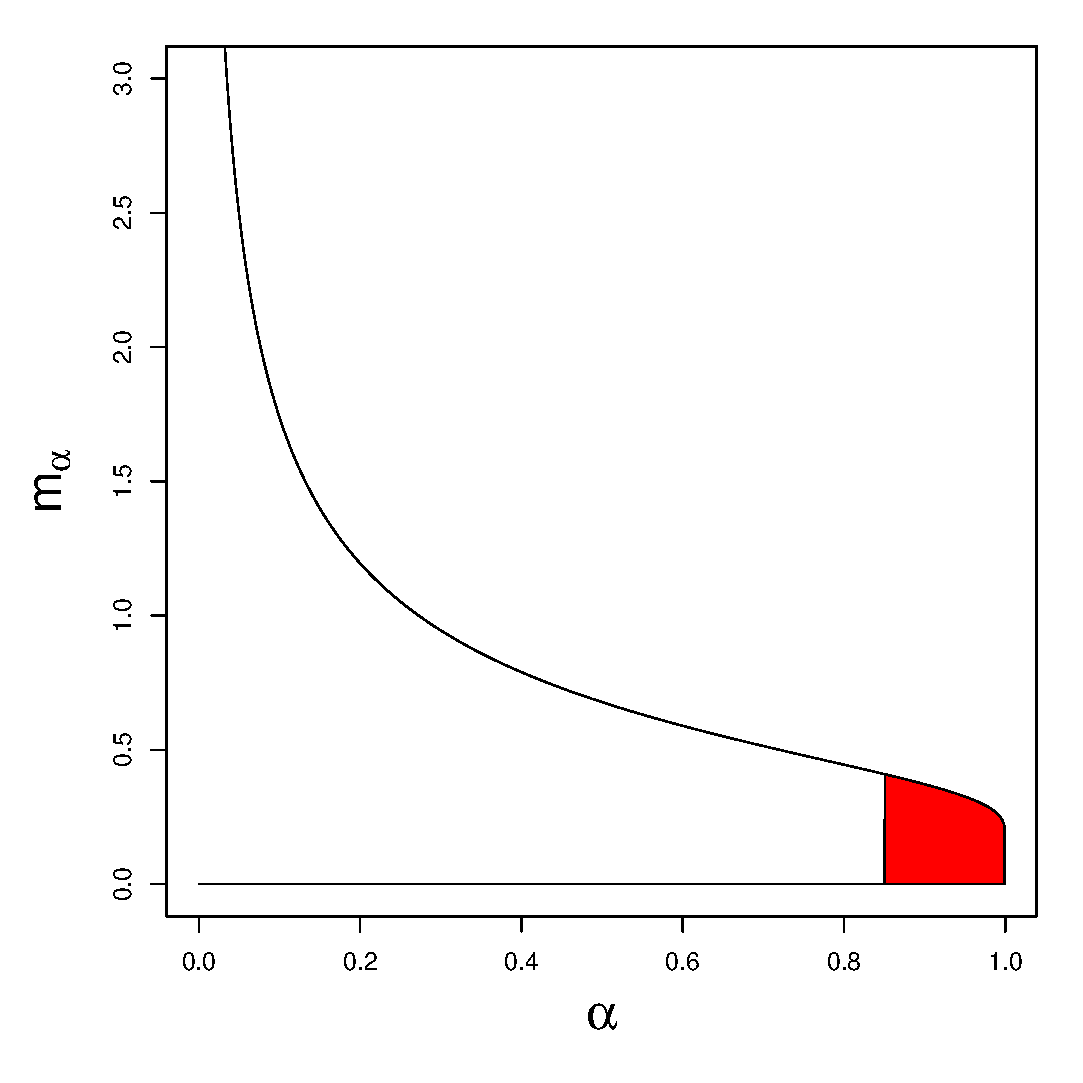
\includegraphics{shortfallcap.eps}}
      \resizebox{60mm}{!}{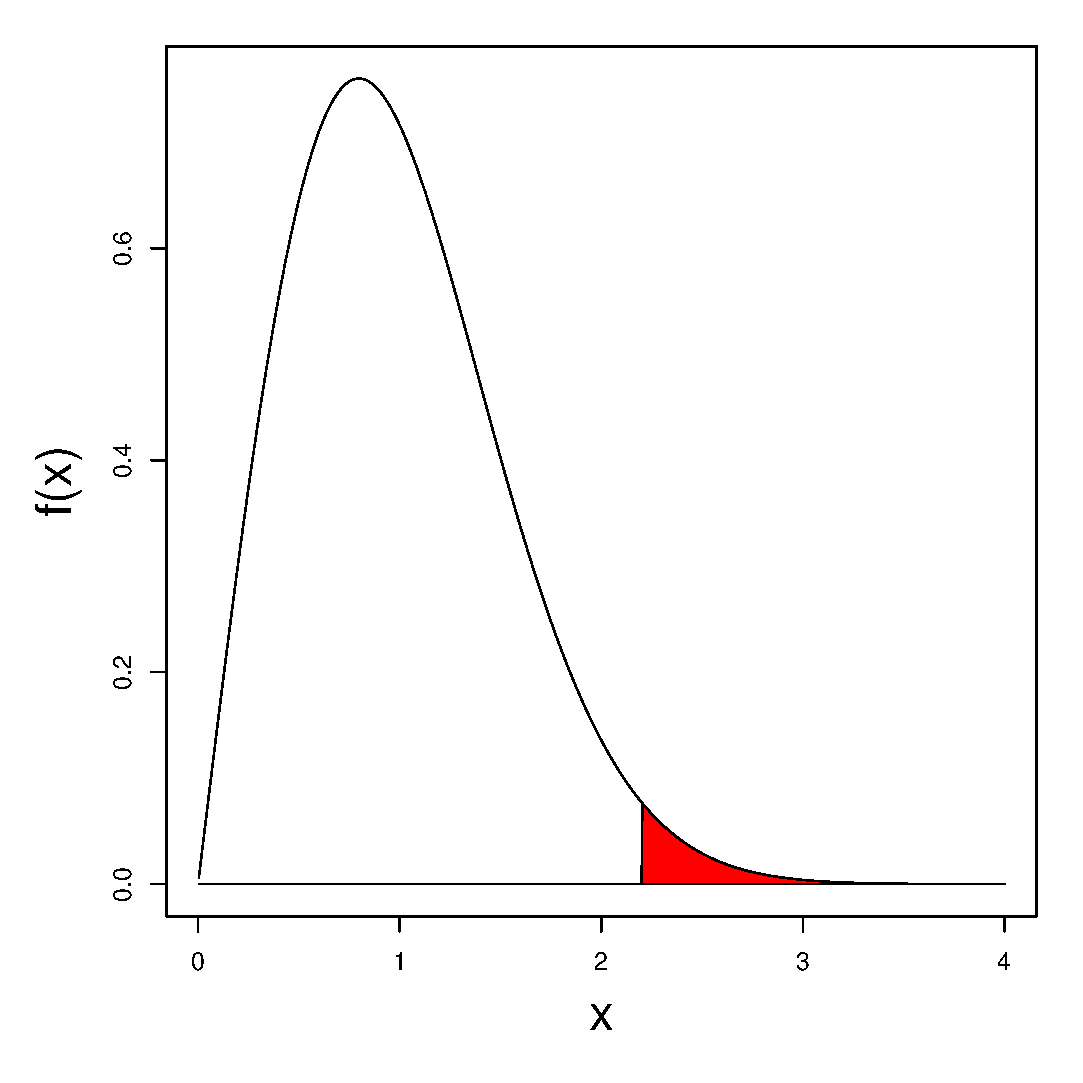
\includegraphics{varcap.eps}} \\
    \end{tabular}
    \caption{The left panel shows capital with fixed expected shortfall (red area under the mean density). The right panel shows capital with fixed shortfall probability (red area under the probability density).}
    \label{fcapital}
  \end{center}
\end{figure}


For an exponential loss distribution, the mean density is flat and \eref{shortfall} reads $1-c=l$ therefore $c=1-l$. For example if expected shortfall is $0.5\%$ of the overall mean loss then  capital is the $99.5\%$ VaR. Setting shortfall probability at $l$ also yields capital $(1-l)$-VaR. Thus fixing expected shortfall and shortfall probability yield identical capital for the exponential loss distribution. For a Pareto loss distribution with increasing mean density, solving \eref{shortfall} yields
$$
\int_c^1 \frac{1}{(1-\alpha)^{1/\gamma}} \de \alpha =
l \int_0^1 \frac{1}{(1-\alpha)^{1/\gamma}} \de \alpha \cq
c=1-l^{\gamma/(\gamma-1)} \;.
$$
In this case capital exceeds $(1-l)$-VaR, and decreases with shape parameter $\gamma$. Generally for an increasing mean density, $M_{[1-l,1]} > lM_{[0,1]}$ thus $c>1-l$, and vice versa for a decreasing mean density. Hence the VaR threshold varies with the shape of the loss distribution. Higher skewness increases the threshold and reduces shortfall probability. Expected shortfall is more superior than shortfall probability when determining capital, since the shape of the loss distribution is reflected in the VaR threshold.

The scale of the loss distribution does not affect the VaR threshold in \eref{shortfall}, since scale factors are present in numerator and denominator. The VaR threshold depends only on the shape parameter and  shortfall proportion $l$. Scale is reflected only when capital is computed from the VaR threshold.




\section{Minimising expected capital surplus and shortfall}

The following sets capital by considering both expected surplus and shortfall. An opportunity cost $j$ is attached to every unit of capital surplus, since surplus is better used in other areas. The corresponding cost of capital shortfall is $k$, for example the borrowing cost under distress. The overall expected cost is
$$
\Gamma = j \left(V_c-M_{[0,c]}\right) + k M_{[c,1]} = k\E\{\max(V_c-x,0)\} + j\E\{\max(x-V_c,0)\} \;,
$$
where $V_c-M_{[0,c]}$ is expected surplus and $M_{[c,1]}$ is expected shortfall. The final expression above is the equivalent standard statistical expression. Setting the derivative of $\Gamma$ with respect to $c$ to zero yields
$$
j(V_c'-m_c)-km_c=0 \cq jc- k(1-c)=0 \cq c=\frac{k}{j+k} = \frac{1}{1+(k/j)^{-1}} \;.
$$
Hence the VaR threshold in this setup increases with the relative unit shortfall cost. If $j=k$ then $c=0.5$, and $c$ increases when $k$ increases relative to $j$. In addition any capital $V_{c^*}$ implies relative shortfall cost $k/j=c^*/(1-c^*)$. For example, $99.5\%$ VaR capital implies $k/j=199$, thus the unit cost of shortfall is approximately $200$ times the unit cost of surplus.




\section{Reinsurance and loss transformation}

Suppose an insurer faces loss $x$, and enters into a reinsurance arrangement whereby a portion $t_\alpha$ of every $\mathrm{VaR}_\alpha$ layer is reinsured and the remaining portion $1-t_\alpha$ is retained. Hence $\mathrm{VaR}_\alpha$ layer and its mean and risk all reduce by $t_\alpha$. The retained loss and the mean and risk densities are, respectively,
\begin{equation}\label{reinsurance}
\tilde{x}\equiv \int_0^1 (x>V_\alpha)(1-t_\alpha) \de V_\alpha \cq
\tilde{m}_\alpha \equiv (1-t_\alpha) m_\alpha \cq
\tilde{r}_\alpha \equiv (1-t_\alpha) r_\alpha \;.
\end{equation}
Risk ratios are unchanged after reinsurance: $\tilde{r}_\alpha/\tilde{m}_\alpha=r_\alpha/m_\alpha$. The loss distribution is altered by reinsurance and is further discussed below.

The set of values of $t_\alpha$ over $0\le \alpha\le 1$ defines the ``reinsurance structure." Typical reinsurance structures are ``quota share": $t_\alpha=t$ and ``excess-of-loss": $t_\alpha=(\alpha> d)$. Quota share covers a constant proportion $t$ of all layers. Excess-of-loss covers all VaR layers above $d$.

The loss distribution after reinsurance is characterised by $\mathrm{VaR}_\alpha$s $\tilde{V}_\alpha$ where $\tilde{V}'_\alpha=(1-t_\alpha)V_\alpha'$. VaR spacings are reduced by the reinsurance applicable to the layer. Applying integration by parts yields
$$
\tilde{V}_\alpha = \int_0^\alpha (1-t_s) V_s' \de s = (1-t_\alpha) V_\alpha +\int_0^\alpha V_s t_s' \de s \;.
$$
For quota share, $t_\alpha'=0$ therefore $\tilde{V}_\alpha=(1-t)V_\alpha$. Losses reduce by a portion $t$. For excess-of-loss, $t_\alpha'=(\alpha=d)$, the Dirac delta function, and $\tilde{V}_\alpha=(\alpha\le d)V_\alpha + (\alpha>d)V_d$. Under this arrangement, all losses below $V_d$ are retained and losses above $V_d$ are capped at $V_d$. Hence the retained loss is $L_{[0,d]}$.

The reinsurance structure can be tailored to yield a target loss distribution or mean and risk density. If the target mean density is $\tilde{m}_\alpha$ then from \eref{reinsurance} the reinsurance structure is $t_\alpha=1-\tilde{m}_\alpha/m_\alpha$. Similarly for a target risk density. If the loss distribution has $\mathrm{VaR}_\alpha$ $\tilde{V}_\alpha$ then $t_\alpha=1-\tilde{V}_\alpha'/V_\alpha'$. In all cases the reinsurance structure computes the ratio between target and original quantities.

Consider a Pareto distributed loss with shape parameter $\gamma>1$ and scale parameter $\beta>0$. Reinsurance is purchased to transform the loss distribution into an exponential with scale $\tilde{\beta}>0$. The reinsurance structure is
$$
t_\alpha = 1-  \frac{\tilde{\beta}(1-\alpha)^{-1} }{\beta\gamma^{-1}(1-\alpha)^{-(1/\gamma+1)}}
= 1-\tilde{\beta}\beta^{-1}\gamma (1-\alpha)^{1/\gamma}
$$
Hence reinsurance is $1-\tilde{\beta}\beta^{-1}\gamma$ at the zero VaR layer, and increases monotonically to $1$ at the highest VaR layer. This result is intuitive since the Pareto is thicker tailed than the exponential. Hence in order to transform the loss from Pareto to exponential, minimum reinsurance is required for small losses and larger losses are increasingly reinsured. Note $\tilde{\beta}\le \beta/\gamma$ since $0\le t_\alpha\le 1$.


\section{Optimal excess-of-loss reinsurance}

Suppose excess-of-loss reinsurance with excess $d$ is purchased. The problem is to calculate an optimal $d$ for the insurer. The retained risk is $R_{[0,d]}$ with unit cost $k$. Reinsurance may be priced in two ways:
\bi

\i Fixed profit margin: reinsurance cost is a margin $\theta$ on the expected loss. The overall cost to the insurer is
$$
\Gamma = k R_{[0,d]} + \theta M_{[d,1]}
$$
with derivative $kr_d-\theta m_d$. Then the optimal $d$ satisfies
$$
\frac{r_d}{m_d} = r_d^* = \frac{d-\Phi(d)}{1-d} = \frac{\theta}{k}
$$
or the risk ratio at $d$ is equal to the ratio between the reinsurer's profit margin and the insurer's unit risk cost. A higher profit margin or lower risk cost increases the excess for the insurer.

\i Risk based pricing: reinsurance cost is a margin $\theta$ on the reinsured risk, and the reinsurer has risk density $\hat{r}_\alpha$. The overall cost to the insurer is
$$
\Gamma = k R_{[0,d]} + \theta \hat{R}_{[d,1]}
$$
with derivative $kR_d-\pi\hat{R}_d$. The optimal $d$ satisfies
$$
kr_d=\theta \hat{r}_d \cq kr_d^*=\theta \hat{r}_d^* \cq k \{d-\Phi(d)\} = \theta \{d-\hat{\Phi}(d)\} \;,
$$
where $\hat{\Phi}$ is the reinsurer's distortion operator.


\ei
In both cases the optimal reinsurance retention is independent of the loss distribution.



\section{Optimal combination of reinsurance and capital}



Suppose XoL reinsurance with threshold $V_c$ is purchased, and capital is set at $V_c$. Hence there is zero shortfall: VaR layers above $c$ are covered by reinsurance, and VaR layers below $c$ are covered by held capital. The problem is to derive an optimal $V_c$ -- the XoL threshold and capital. Holding capital involves servicing cost, at $\pi$ per unit. The reinsurer charges a loading equal to the risk of the $[c,1]$-VaR layer. These yield an overall cost
$$
p(c)= \left\{ \pi V_c + \E\left(\ell_{[0,c]}\right)  \right\} + \left\{ \int_c^1 r_\alpha \de \alpha +  \E\left(\ell_{[c,1]}\right) \right\}
=\E(x) + \pi V_c +  \int_c^1 r_\alpha \de \alpha \;,
$$
and the derivative with respect to $c$ is
$$
 p'(c)=\pi V'_c - r_c = V'_c\left\{\pi-c+\Phi(c) \right\}
$$
hence the payout is minimise when $c$ satisfies $c-\Phi(c)=\pi$. The optimal XoL purchase and capital buffer do not depend on the loss distribution, only on the distortion operator $\Phi$.


\section{Combining quota share and excess-of-loss reinsurance}

Suppose a combination of quota share and excess-of-loss reinsurance is deployed. The aim is to minimise cost subject to retained mean loss $M$. Hence minimise
$$
\Gamma = k(1-t)r_{[0,d]} +j_1 r_{[d,1]} + j_2 tr_{[0,d]}
-\lambda \left\{ (1-t)m_{[0,d]} - M \right\}
$$
where $t$ and $d$ are parameters of quota share and excess-of-loss reinsurance, respectively. In addition $k$, $j_1$ and $j_2$ are respective cost per unit risk for the insurer, excess-of-loss and quota share reinsurers. $\lambda$ is the Lagrange multiplier.

The solutions $t$, $d$ and $\lambda$ are
$$
t=xxx \cq d=xxx \cq \lambda =xxx \;.
$$




\newpage

\bibliography{PhD}



\end{document}
